The hull force components from the wPCC VCT as well as predictions with the identified model for the drift angle tests are shown in \autoref{fig:drift_angle_wPCC}. The total damping forces $X_D$, $Y_D$, and $N_D$ are the sum of the components from the hull (H), rudder (R) and propellers (P). Both the hull and the rudder contribute to the total sway force as shown in \autoref{fig:drift_angle_Y}. The hull yawing moment is close to zero for drift angles up to 10 degrees as shown in \autoref{fig:drift_angle_N}. This means that the total hull yawing moment acting on the ship, is only generated by the inviscid Munk moment -- which is not included in $N_H$. A nonlinear viscous contribution is present for larger drift angles. The rudders are however the main contributors to the viscous yawing moment.   
\begin{figure}[h]
     \centering
     \begin{subfigure}[b]{0.49\textwidth}
         \centering
         \includesvg{figures/results_wPCC_VCT.drift_angle_X.svg}
        \caption{Surge force.}
        \label{fig:drift_angle_X}
     \end{subfigure}
     \hfill
     \begin{subfigure}[b]{0.49\textwidth}
         \centering
         \includesvg{figures/results_wPCC_VCT.drift_angle_Y.svg}
        \caption{Sway force.}
        \label{fig:drift_angle_Y}
     \end{subfigure}
     \vfill
     \begin{subfigure}[b]{0.49\textwidth}
         \centering
         \includesvg{figures/results_wPCC_VCT.drift_angle_N.svg}
        \caption{Yawing moment.}
        \label{fig:drift_angle_N}
     \end{subfigure}
    \caption{wPCC hull forces for combined circle and drift angle tests from VCT (dots) and predictions (lines) with the hull force model.}
    \label{fig:drift_angle_wPCC}
\end{figure}
\begin{figure}[h]
     \centering
     \begin{subfigure}[b]{0.49\textwidth}
         \centering
         \includesvg{figures/results_wPCC_VCT.circle_drift_Y_H.svg}
        \caption{Sway force.}
        \label{fig:circle_drift_Y_H}
     \end{subfigure}
     \hfill
     \begin{subfigure}[b]{0.49\textwidth}
         \centering
         \includesvg{figures/results_wPCC_VCT.circle_drift_N_H.svg}
        \caption{Yawing moment.}
        \label{fig:circle_drift_N_H}
     \end{subfigure}
    \caption{Force components from VCT (dots) and predictions (lines) with the semi-empirical model for the wPCC drift angle tests.}
    \label{fig:overshoots_wPCC}
\end{figure}

The flow from the port dagger board hits the starboard rudder for 15 degrees drift angle as shown in \autoref{fig:streamlines15}.
\begin{figure}[h]
    \centering
    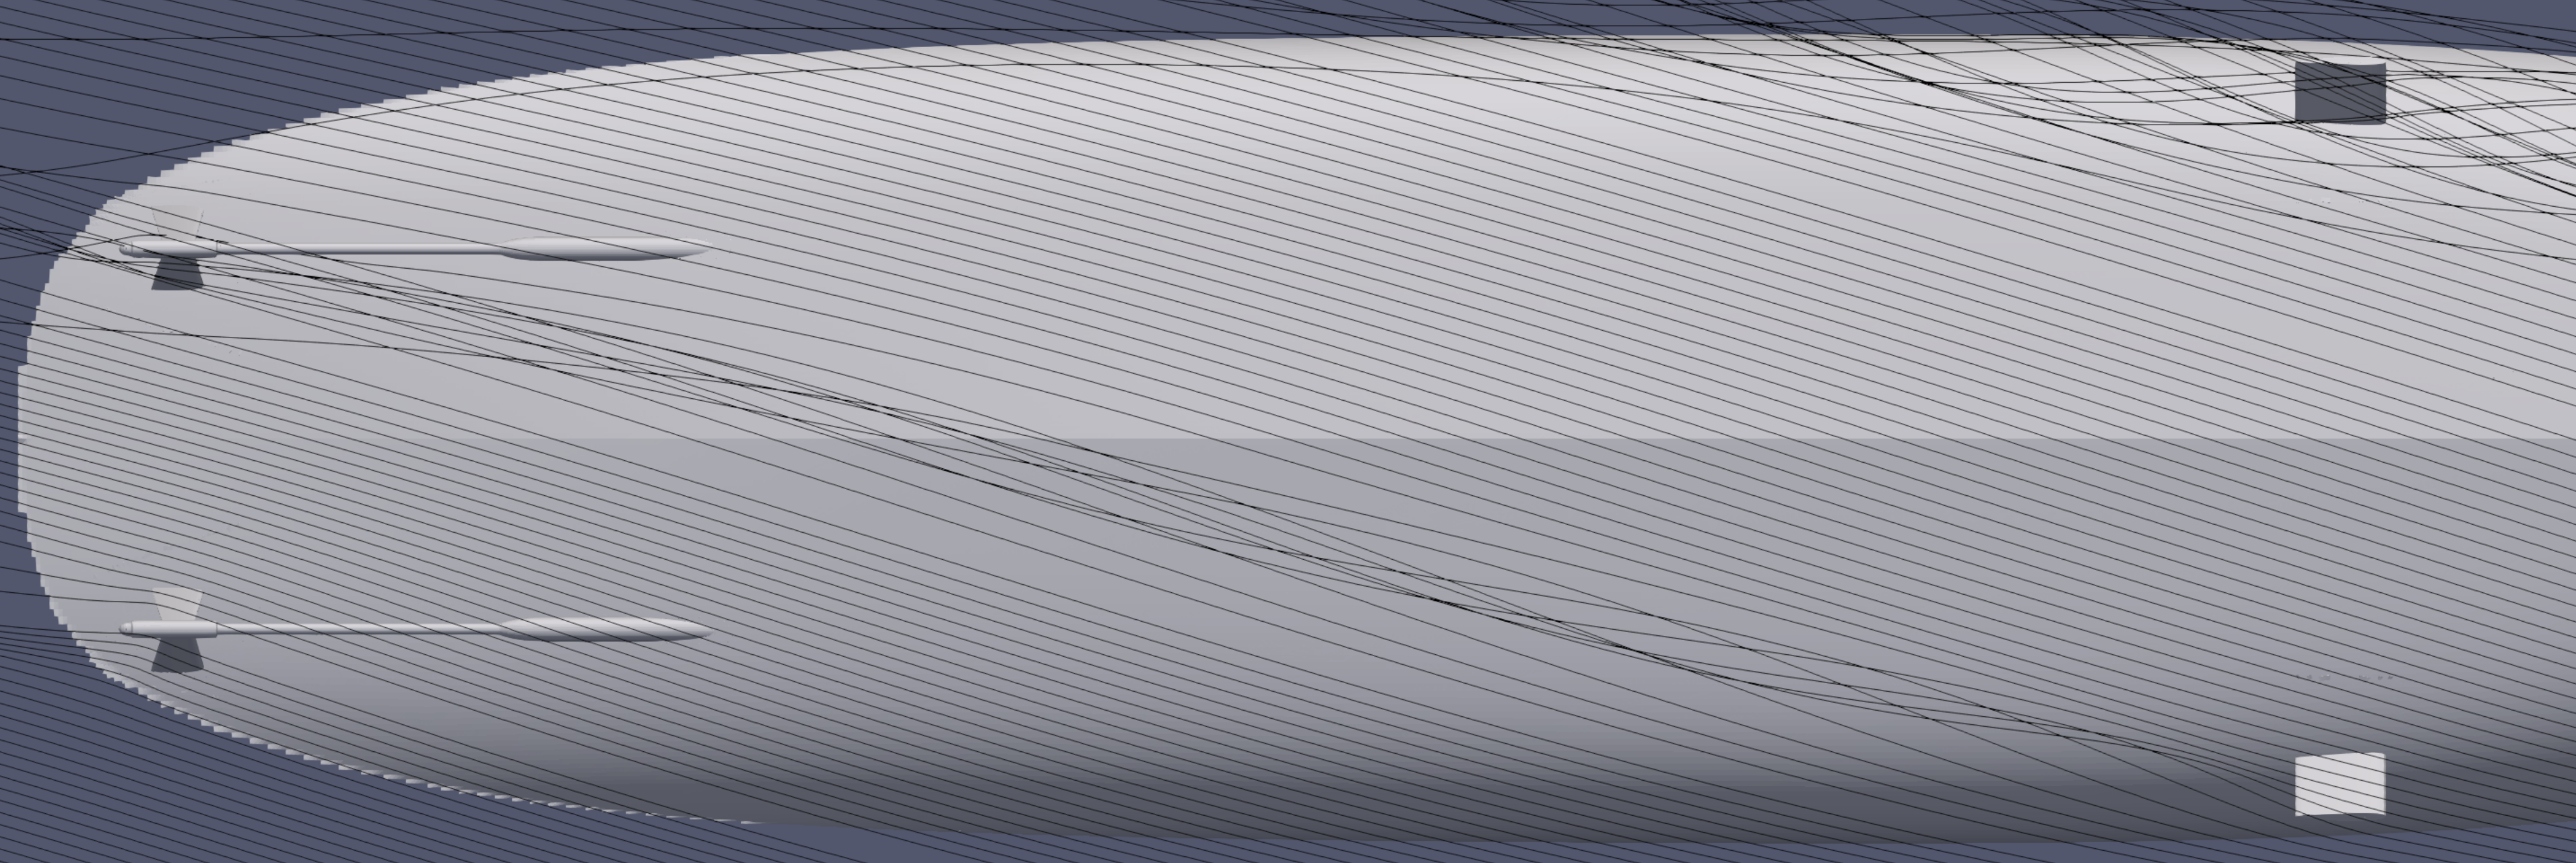
\includegraphics[width=\textwidth]{figures/paraview_drift_15.png}
    \caption{Streamlines for wPCC at 15 degrees drift angle.}
    \label{fig:streamlines15}
\end{figure}